\documentclass{article}
\usepackage[utf8]{inputenc}
\usepackage{apacite}
\usepackage{graphicx}   
\graphicspath{{figures/}}

\title{Augmented Reality and the Piano: A Review of Immersive Learning Technologies}
\author{Jordan Aiko Deja, Matjuž Kljun, Klen Čopič Pucihar and Aaron Quigley}
\begin{abstract}

% this abstract might not make any sense anymore 
     Learning and mastering the piano involves several years of practice and hardwork. Throughout the years, several works have been designed and developed to help novices learn, and help teachers teach the piano. In this survey, we look at the different novel approaches that have been created to in learning the piano with the use of Augmented Reality. We put specific focus on breakthrough innovations on giving feedback, correcting learner mistakes and helping finger positioning. We intend to inquire on technologies needed that bridge novices closer into becoming experts. We also discuss possible takeaways and future steps towards pushing the said domain further. 
     
\end{abstract}
\date{February 2020}

\begin{document}

\maketitle

\section{Links I need}

https://www.musicbusinessworldwide.com/jean-michel-jarre-launches-infinite-music-app-eon/

Piano Training System (Ubicomp)
https://www.youtube.com/watch?v=4ohSTRXjBNI




UbiComp Piano - say what you want to say 
\cite{Weing:2013:PEI:2494091.2494113}


\section{Papers to include}

\nocite{*}

\citeP{poupyrev2000augmented}
\citeP{santos2013augmented}


\cite{ARPiano-2018} - ARPiano 

Rhythm Games and Piano 

Augmented reality learning experiences: Survey of prototype design and evaluation

\section{Introduction}

\section{Marker-Dependent Augmented Reality Music Learning}

\begin{figure}
    \centering
    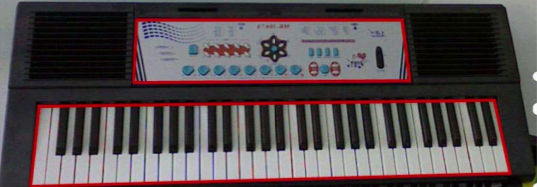
\includegraphics[width=15cm]{figures/pianomarker.png}
    \caption{Piano Augmented Reality marker}
    \label{fig:pianomarker}
\end{figure}



\section{Head-Mounted Augmented Reality Music Learning}

\begin{figure}
    \centering
    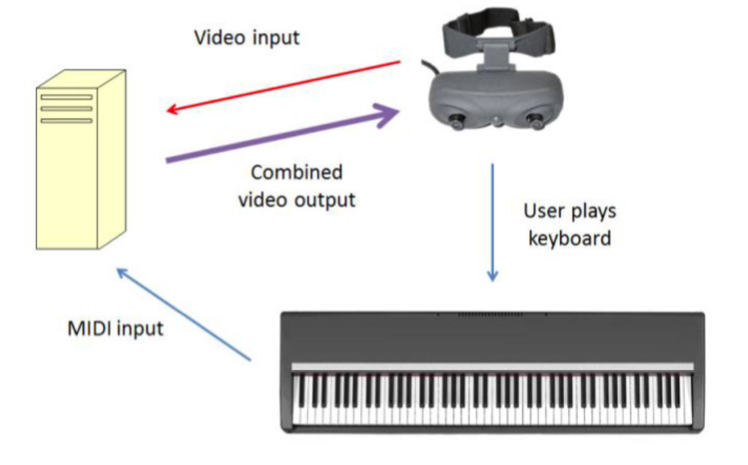
\includegraphics[width=10cm]{figures/headmountedpiano1.png}
    \caption{Architecture of the Head Mounted Piano by cite! }
    \label{fig:pianoheadmountedarch}
\end{figure}

\begin{figure}
    \centering
    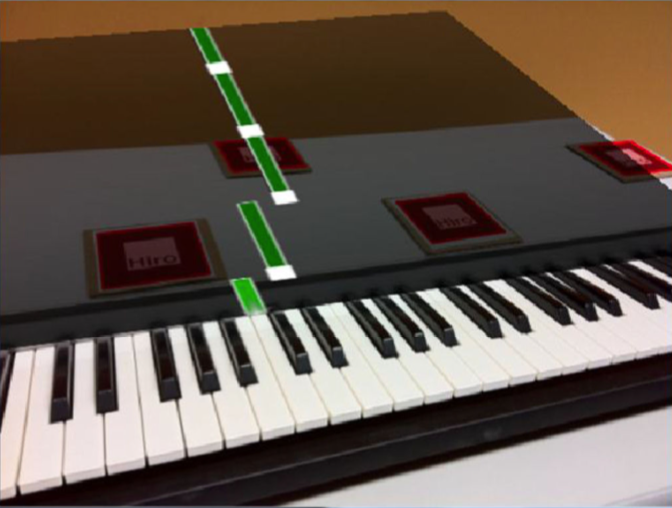
\includegraphics[width=10cm]{figures/headmountedview.png}
    \caption{View from the Head Mounted Piano AR  }
    \label{fig:View from the HeadMounted}
\end{figure}


\section{Agent-based Augmented Reality Music Learning}


\section{Augmented Reality Music Learning Using Interactive Visualizations}

\begin{figure}
    \centering
    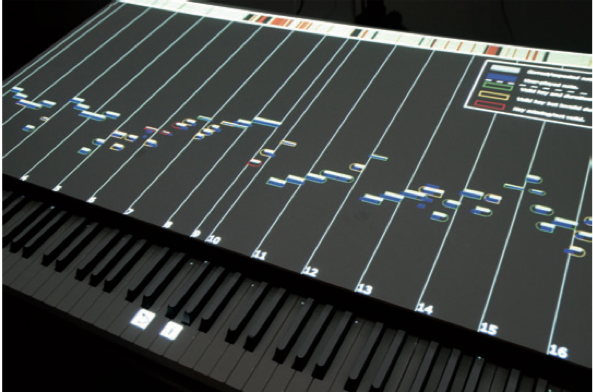
\includegraphics[width=10cm]{figures/piano}
    \caption{View of the Detailed Screen of P.I.A.N.O.› }
    \label{fig:View from the HeadMounted}
\end{figure}



\section{Review of Augmented Reality Music Learning Experiences}



\section{Future Work}


% overview of audio augmented reality
% classical works in audio augmented reality
% visualizations in audio
% audio and lighting effects in performance media
% usability studies involving audio augmented reality
% novel works and audio ar on inclusive music (for def or pwd)




% music features and visualization

% taxonomy of AR and music 

% music decorates space by andre
% using visualization 




\bibliographystyle{apacite}
\bibliography{references}

\end{document}
